\section{Développement Java : Outil de gestion de tests pour un constructeur automobile}
La pemière partie de mon stage a été occupé par beaucoup de développement en Java. L'idée de cette part du stage était de participer aux contrats remplis par Alter Frame et avoir ainsi une idée précise d'à quoi ressemblait le travail dans l'entreprise. Je vais profiter de cette partie pour résumer les projets auxquels j'ai participé et dans quelle mesure, sans pour autant le commanditaire dans un soucis de discrétion.

\subsection{Le contexte}
Produire et mettre en vente une voiture requière que celle-ci soit passée par une batterie de tests intensifs. Ce premier projet était un logiciel permettant de gérer ces tests de bout en bout : ajouter un véhicule à la base de données, établir une liste d'organes à tester, une liste de tests pour chaque organe, puis ensuite enregistrer les résultats des tests qui ont été effectués (voir graphique~\ref{fig:acceuil}). Cela représente le c\oe{}ur de la logique métier impliquée dans le logiciel, mais naturellement il y avait autour de ce noyau de nombreuses fonctionnalités plus ``classiques'' telles que la gestion d'authentification des utilisateurs, les différents privilèges (administrateur, utilisateur simple), etc.

\begin{figure}{l}
	\makebox[\textwidth][c]{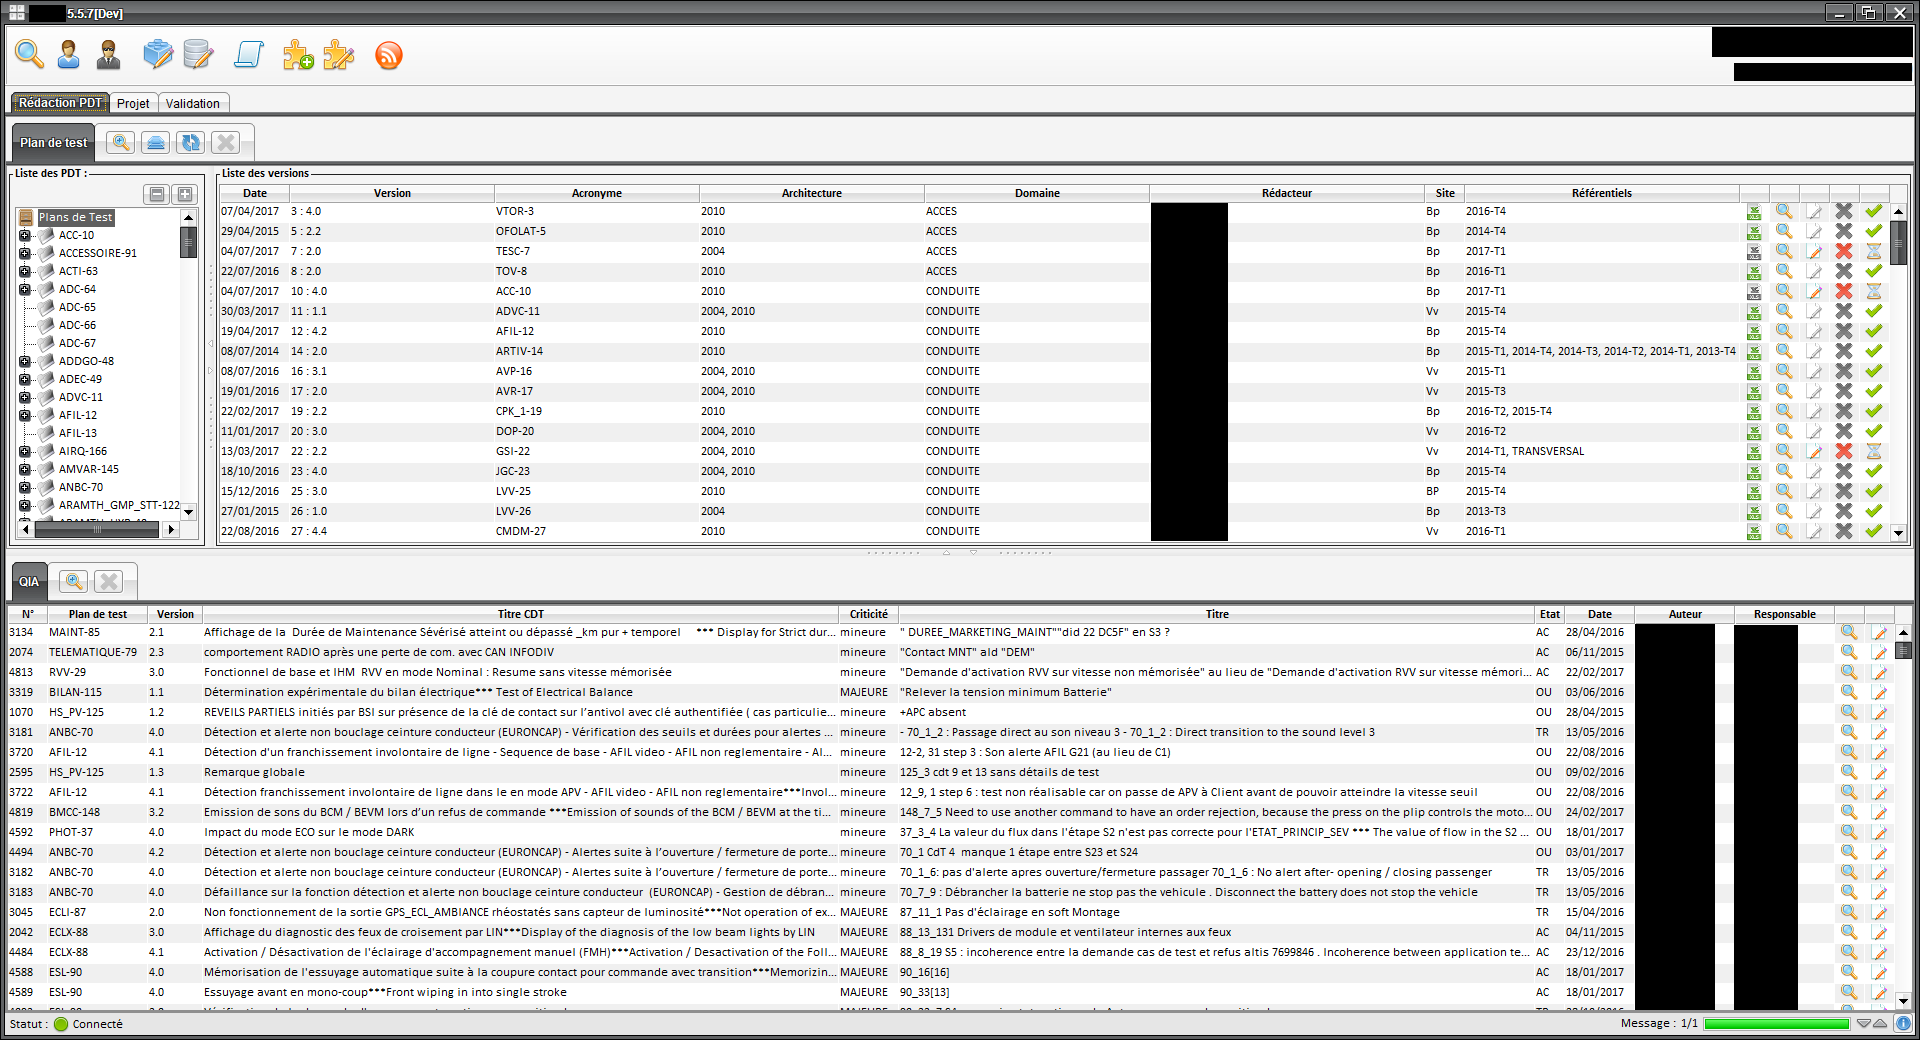
\includegraphics[width=\paperwidth]{images/attm_acceuil}}
	\caption{Fenêtre de démarrage de l'outil}
	\label{fig:acceuil}
\end{figure}

De manière intéressante, j'ai remarqué en travaillant sur le workflow des tests automobile implémenté dans cet outil que celui-ci est semblable au cycle en V qui fait partie intégrante de la gestion de projet en informatique. Les détails étaient, naturellement, très différents mais ce qui semblait être les grandes lignes de la façon dont un projet de tests devait être géré était au contraire très proche de ce que nous connaissons dans le monde de l'informatique.

Une particularité de ce projet est qu'il s'agit d'un logiciel déjà existant qui a été récupéré par Alter Frame pour de la mise à jour et de la maintenance. L'ESN initialement en charge du projet avait perdu le contrat et mon travail a, de ce fait, été majoritairement constitué de correction de bugs et, dans une moindre mesure, d'ajout de fonctionnalités mineures (voir section~\ref{subsec:ajout}).

\subsection{Environnement technique}
\begin{itemize}[label=$\bullet$]
	\item \emph{Java 7 :} Le projet étant vieux de plusieurs années déjà, il utilise la version de Java qui était en vigueur à l'époque de sa genèse à savoir Java 7.
	\item \emph{Java Swing\cite{swing_wiki} :} Pour les mêmes raisons que Java 7, le framework utilisé pour la partie graphique de l'application est Java Swing.
	\item \emph{Apache ActiveMQ\cite{activemq} :} L'outil fonctionne selon une architecture client-serveur classique et la communication entre le serveur et les différents clients se fait au-travers d'un système de queues et du système open source ActiveMQ.
	\item \emph{MyBatis\cite{mybatis} :} La liaison base de données/application se fait grâce à cet ORM open source qui a la particularité de mapper des méthodes Java à des requêtes SQL\cite{mybatis_prez}.
\end{itemize}

\subsection{Fonctionnalités ajoutées}
\label{subsec:ajout}
Comme mentionné plus haut, le gros du travail sur cet outil consistait à reprendre et débugger un code au départ écrit par une autre société. Il s'agissait donc tout à la fois de trouver des erreurs, améliorer ce qui pouvait l'être (notamment en termes de performances) et comprendre intrinséquement le fonctionnement de l'application. Tout cela représente un temps de développement considérable.

Les fonctionnalités ajoutées sont donc, comparativement, peu nombreuses. Ma première réalisation originale sur ce projet a été de modifier la génération de tableau Excel (voir figure~\ref{fig:classeur}) pour prendre en compte de nouvelles spécifications.

\begin{figure}{l}
	\makebox[\textwidth][c]{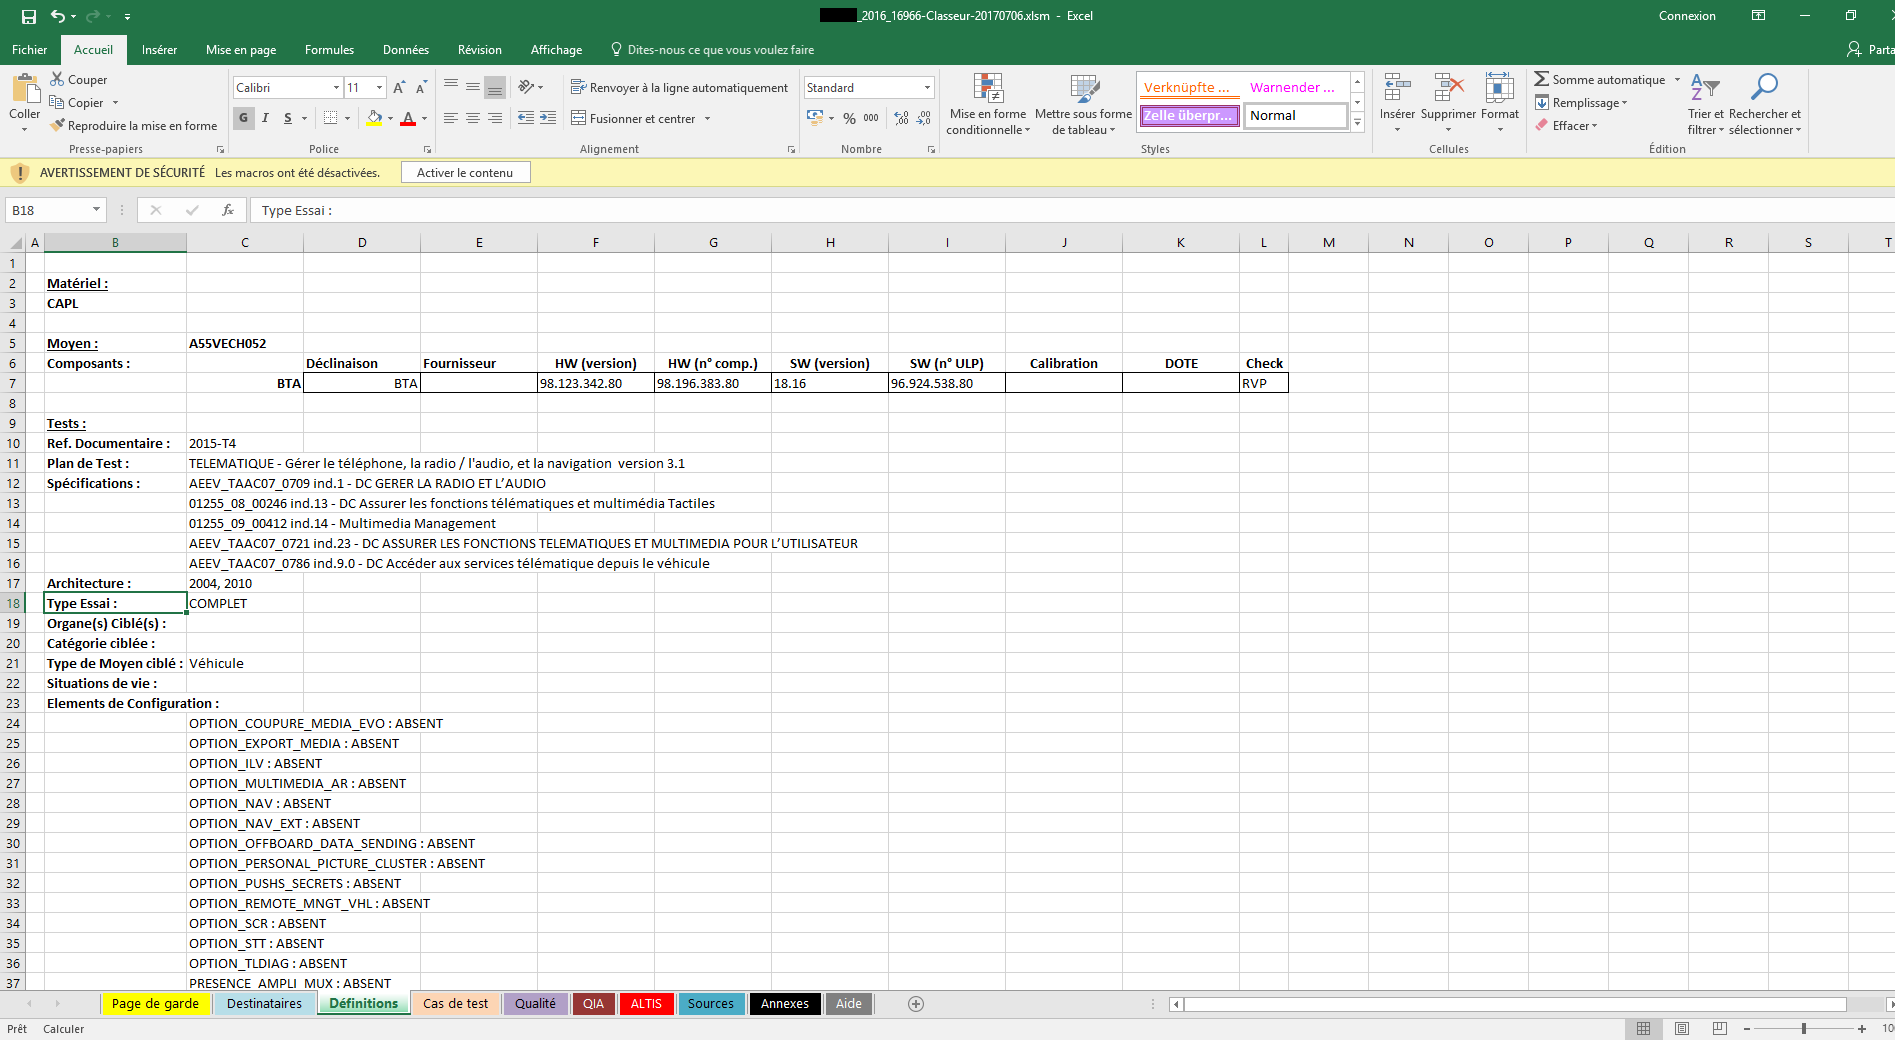
\includegraphics[width=\paperwidth]{images/attm_classeur}}
	\caption{Classeur Excel généré par l'outil}
	\label{fig:classeur}
\end{figure}

La génération en elle-même existait déjà à ce moment à l'aide de Microsoft Visual Basic, Scripting Edition\cite{vbscript}\footnote{VBScript pour les intimes}. Ce qui était demandé par le client était d'ajouter une nouvelle catégorie d'informations à ce classeur, à savoir les \emph{Situations de vie}.

%TODO : INSÉRER UNE EXPLICATION ET DES EXTRAITS DE CODE